RHODES approach to traffic signal optimization is a hierachical one with 3 layers of detail, see figure \ref{fig:rhodes_hierarchi}. They can be rougly be summarized accordingly:

\begin{enumerate}
\item The macroscopic layer performs \textit{dynamic network loading}, which involves observing changes in the aggregated flow data of the entire network due to variations in the OD matrices. This layer supplies estimates of link flows to the middle level in rough numbers eg. vehicles per hour.
\item The mesoscopic middle layer considers sectors of the network eg. an arterial. This \textit{network flow control} layer work in the detail level of platoons and average speeds. Green time is allocated to phases to accomodate the movements of the platoons and so coordination of signals is done at this level.
\item At the lowest level is \textit{intersection control} where vehicles are handled individually (a microscopic layer). Here the green times and phase ordering suggested by the middle layer are fine tuned.
\end{enumerate}

\begin{figure}[!ht]
\begin{center}
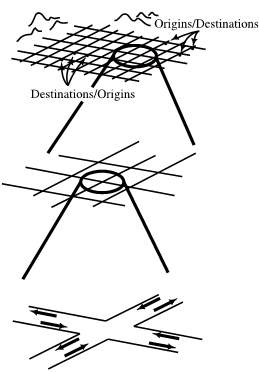
\includegraphics[scale=0.5]{rhodes_hierachy.png} 
\end{center}
\caption{The three levels of detail: network, sector, and intersection}
\label{fig:rhodes_hierarchi}
\end{figure}

An adaptive traffic control system must operate quickly in order to adapt signals to traffic in real-time. The RHODES platform has good decomposition opportunities and is pluggable ie. the upper level is a black box feeding the lower level with predictions and optimizations.

\subsubsection*{Detection}
Detections methods are not discussed in detail in the paper. They can be of any technology including induction loops and video. 

Each link facing an intersection under intersection control are fitted with detectors to give the prediction methods optimum operating conditions. Detectors are placed in the beginning of the link so that the prediction method can use a longer horizon.

\begin{figure}[!ht]
\begin{center}
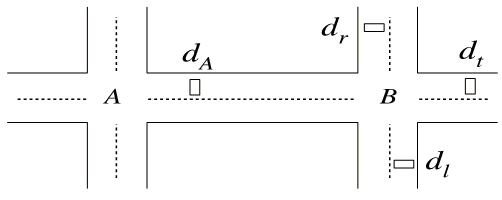
\includegraphics[scale=0.5]{rhodes_prediction-strategy.png} 
\end{center}
\caption{Detector placement and propogation of information in a simple grid}
\label{fig:rhodes_predict}
\end{figure}

\subsubsection*{Prediction}
The PREDICT method by the co-author, Head, is used to make predictions for individual vehicles. PREDICT is build for network prediction and relies on the fact that incoming flow to an intersection originates from adjacent intersections. This concept can be explained from figure \ref{fig:rhodes_predict} where traffic detected at $d_a$ is the sum of right-turning traffic at detector $d_r$, left turning traffic at $d_l$ and through-going traffic at $d_t$.

Thus given flow estimates for the links facing intersection B and turning probabilities for each link and estimate can be given for the inflow to intersection A from east. On the link between the two intersections there will be traffic entering and exiting the system, but these contributions - and losses - to the traffic, which can be measured at $d_a$ are expected to be very small.

Prediction of arrival times of the vehicles which has passed detectors $d_{\lbrace r,t,l \rbrace}$ depend on the current phase at intersection B and queue conditions. Mirchandani and Head has identified four cases, which cover arrivals to an intersection, which are summarized in table \ref{tbl:delaycases}.

\begin{table}[!ht]
\begin{center}
\begin{tabular}{l|ll}
 & \textbf{Green} & \textbf{Red} \\ \hline
\textbf{No queue} & 0 & $T_G$ \\
\textbf{Queue} & $T_Q$ & $T_G$ + $T_Q$
\end{tabular}
\end{center}
\caption{Delay incurred for a vehicle arriving to an intersection in various states where $T_Q$ is the time for ahead queue to clear and $T_G$ is the time to the next green.}
\label{tbl:delaycases}
\end{table}

In the cases involving queue there is, of course, a possibility that the vehicle will not be able to cross the intersection before several green phases have occured. This sometimes happens under high congestion.

\subsubsection*{Optimization}

\subsubsection*{Evaluation}
